\documentclass[11pt,oneside]{article}
\input{coursHeadings}

\usepackage[%
    pdftitle={TD Communication technique},
    pdfauthor={Xavier Pessoles},
    colorlinks=true,
    linkcolor=blue,
    citecolor=magenta]{hyperref}



% \makeatletter \let\ps@plain\ps@empty \makeatother
%% DEBUT DU DOCUMENT
%% =================
\sloppy
\hyphenpenalty 10000

\newcommand{\Pointilles}[1][3]{%
\multido{}{#1}{\makebox[\linewidth]{\dotfill}\\[\parskip]
}}


\begin{document}


\newboolean{prof}
\setboolean{prof}{false}
%------------- En tetes et Pieds de Pages ------------
\pagestyle{fancy}
\renewcommand{\headrulewidth}{0pt}

\fancyhead{}
\fancyhead[L]{%
\begin{minipage}[c]{1.6cm}
\includegraphics[width=2cm]{png/logo_ptsi.png}%
\end{minipage}
\rule{2cm}{.5pt}
}

\fancyhead[C]{\rule{11cm}{.5pt}}

\fancyhead[R]{%
\begin{minipage}[c]{3cm}
\begin{flushright}
\footnotesize{\textit{\textsf{Sciences Industrielles\\ pour l'Ingénieur}}}%
\end{flushright}
\end{minipage}
}

\renewcommand{\footrulewidth}{0.2pt}

\fancyfoot[C]{\footnotesize{\bfseries \thepage}}
\fancyfoot[L]{\footnotesize{2012 -- 2013} \\ X. \textsc{Pessoles}}
\ifthenelse{\boolean{prof}}{%
\fancyfoot[R]{\footnotesize{TD -- CI 5 : Communication technique -- P}}
}{%
\fancyfoot[R]{\footnotesize{TD -- CI 5 : Communication technique}}
}


%\begin{center}
%\textit{Centre d'intérêt}
%\end{center}


\begin{center}
 \huge\textsc{CI 5 -- Communication technique}
\end{center}

\begin{center}
 \LARGE\textsc{Représentation des pièces mécaniques}
\end{center}


\begin{center}
 \LARGE\textsc{PINCE SCHRADER}
\end{center}

\vspace{.5cm}

\textit{D'après documents de Renan Bonnard}

\begin{contexte}
\begin{itemize}
\item Contexte technique : représentation de pièces géométriques diverses
\item Objectifs : 
\begin{itemize}
\item savoir passer d'une représentation 3D à une représentation 2D en respectant les normes de représentation;
\item identifier des composants dans un dessin d'ensemble
\end{itemize}
\end{itemize}
\end{contexte}

\section*{Mise en situation}
\begin{center}
\includegraphics[width=.9\textwidth]{png/fig1}
\end{center}

La pince Schrader est un préhenseur équipant certains bras de robot. Afin de s’adapter au type
d’objet à saisir/maintenir, les doigts de la pince peuvent recevoir différents types de supports.
La pince et est alimentée par de l’air sous pression pouvant aller de 2 à 10 bars.

\begin{minipage}[c]{.45\linewidth}
\begin{center}
\includegraphics[width=\textwidth]{png/fig2}
\end{center}
\end{minipage} \hfill
\begin{minipage}[c]{.45\linewidth}
\begin{center}
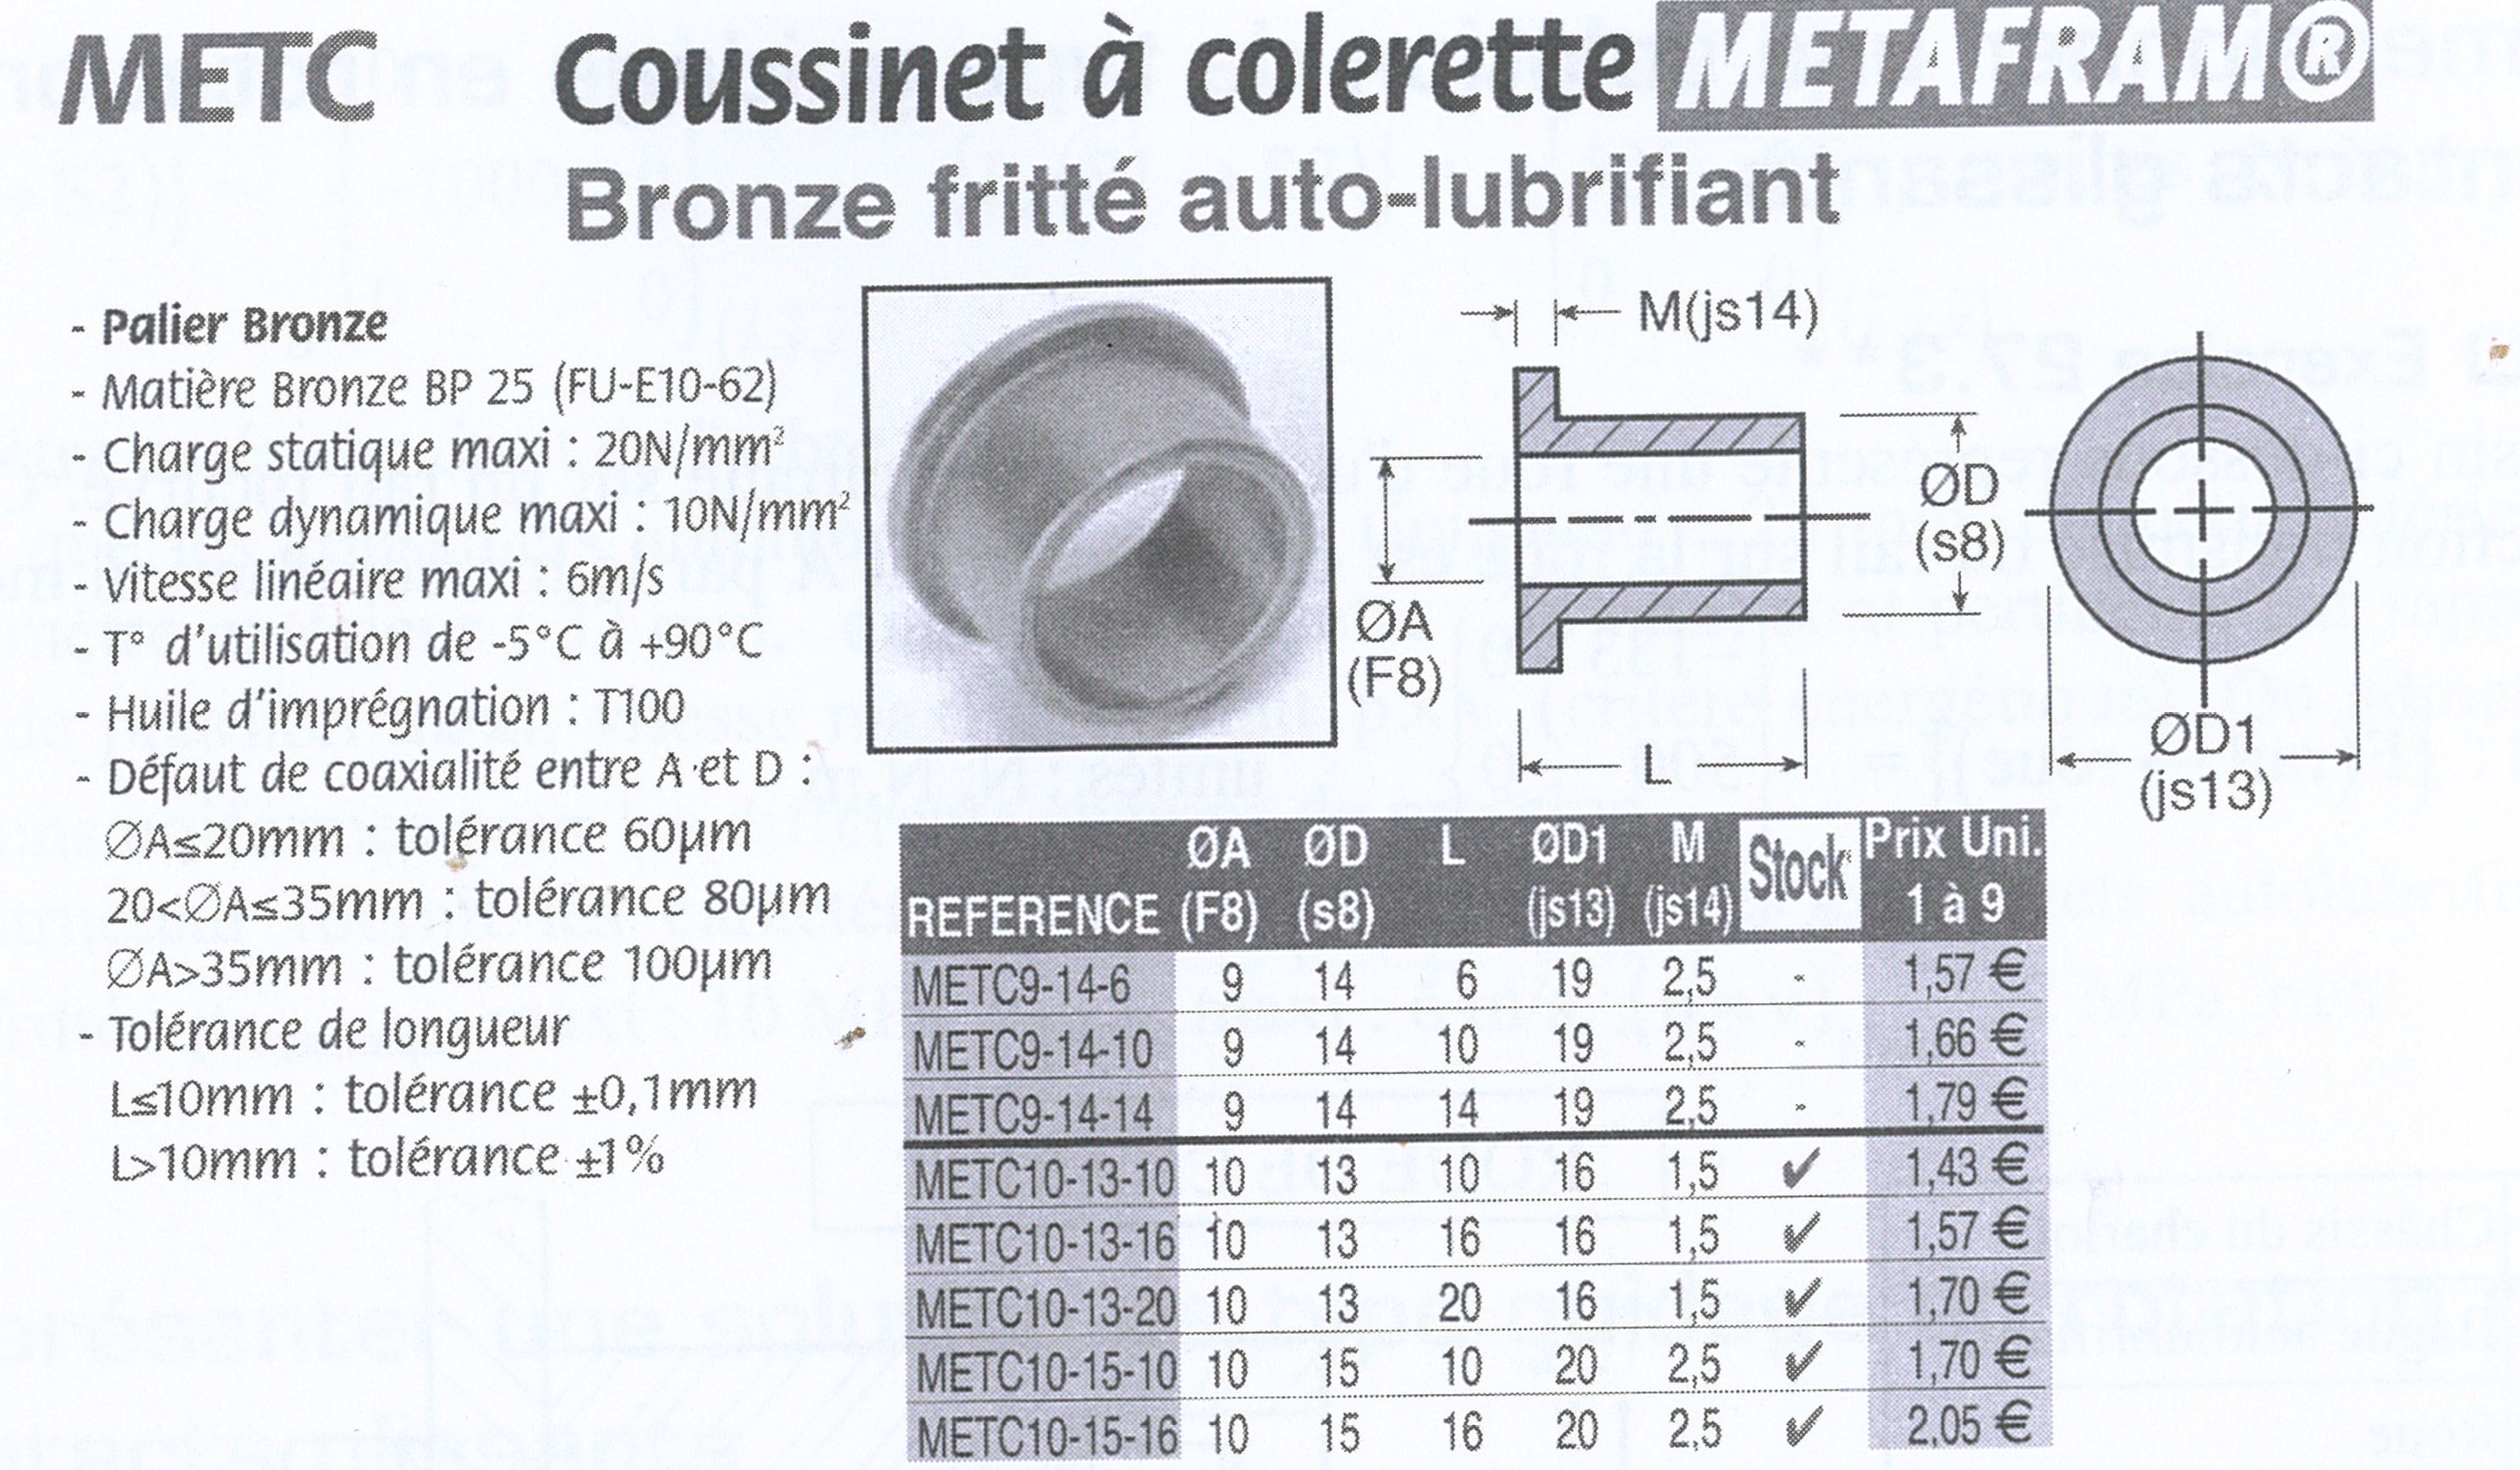
\includegraphics[width=\textwidth]{png/fig3}
\end{center}
\end{minipage}

\section*{Fonctionnement}

\begin{minipage}[c]{.7\linewidth}
Le dessin d'ensemble et la maquette numérique fournis
représentent la pince de préhension du robot Schrader. Elle permet,
à partir d'une source d'énergie pneumatique à laquelle elle est
reliée, de saisir une pièce grâce à deux doigts 7a et 7b. Pour cela,
l’air sous pression pénètre dans la chambre cylindrique du corps 1,
poussant ainsi le piston qui effectue un mouvement de translation
dans la chambre. Par l’intermédiaire des biellettes 4, la translation
du piston entraîne une rotation des doigts 7a et 7b autour des axes
de doigts 8a et 8b. On obtient ainsi la fermeture de la pince,
nécessaire à la prise et au maintien de la pièce. L’ouverture de la
pince est obtenue à l’aide des deux ressorts 6a et 6b.
\end{minipage}
\begin{minipage}[c]{.25\linewidth}
\hfill
\begin{center}
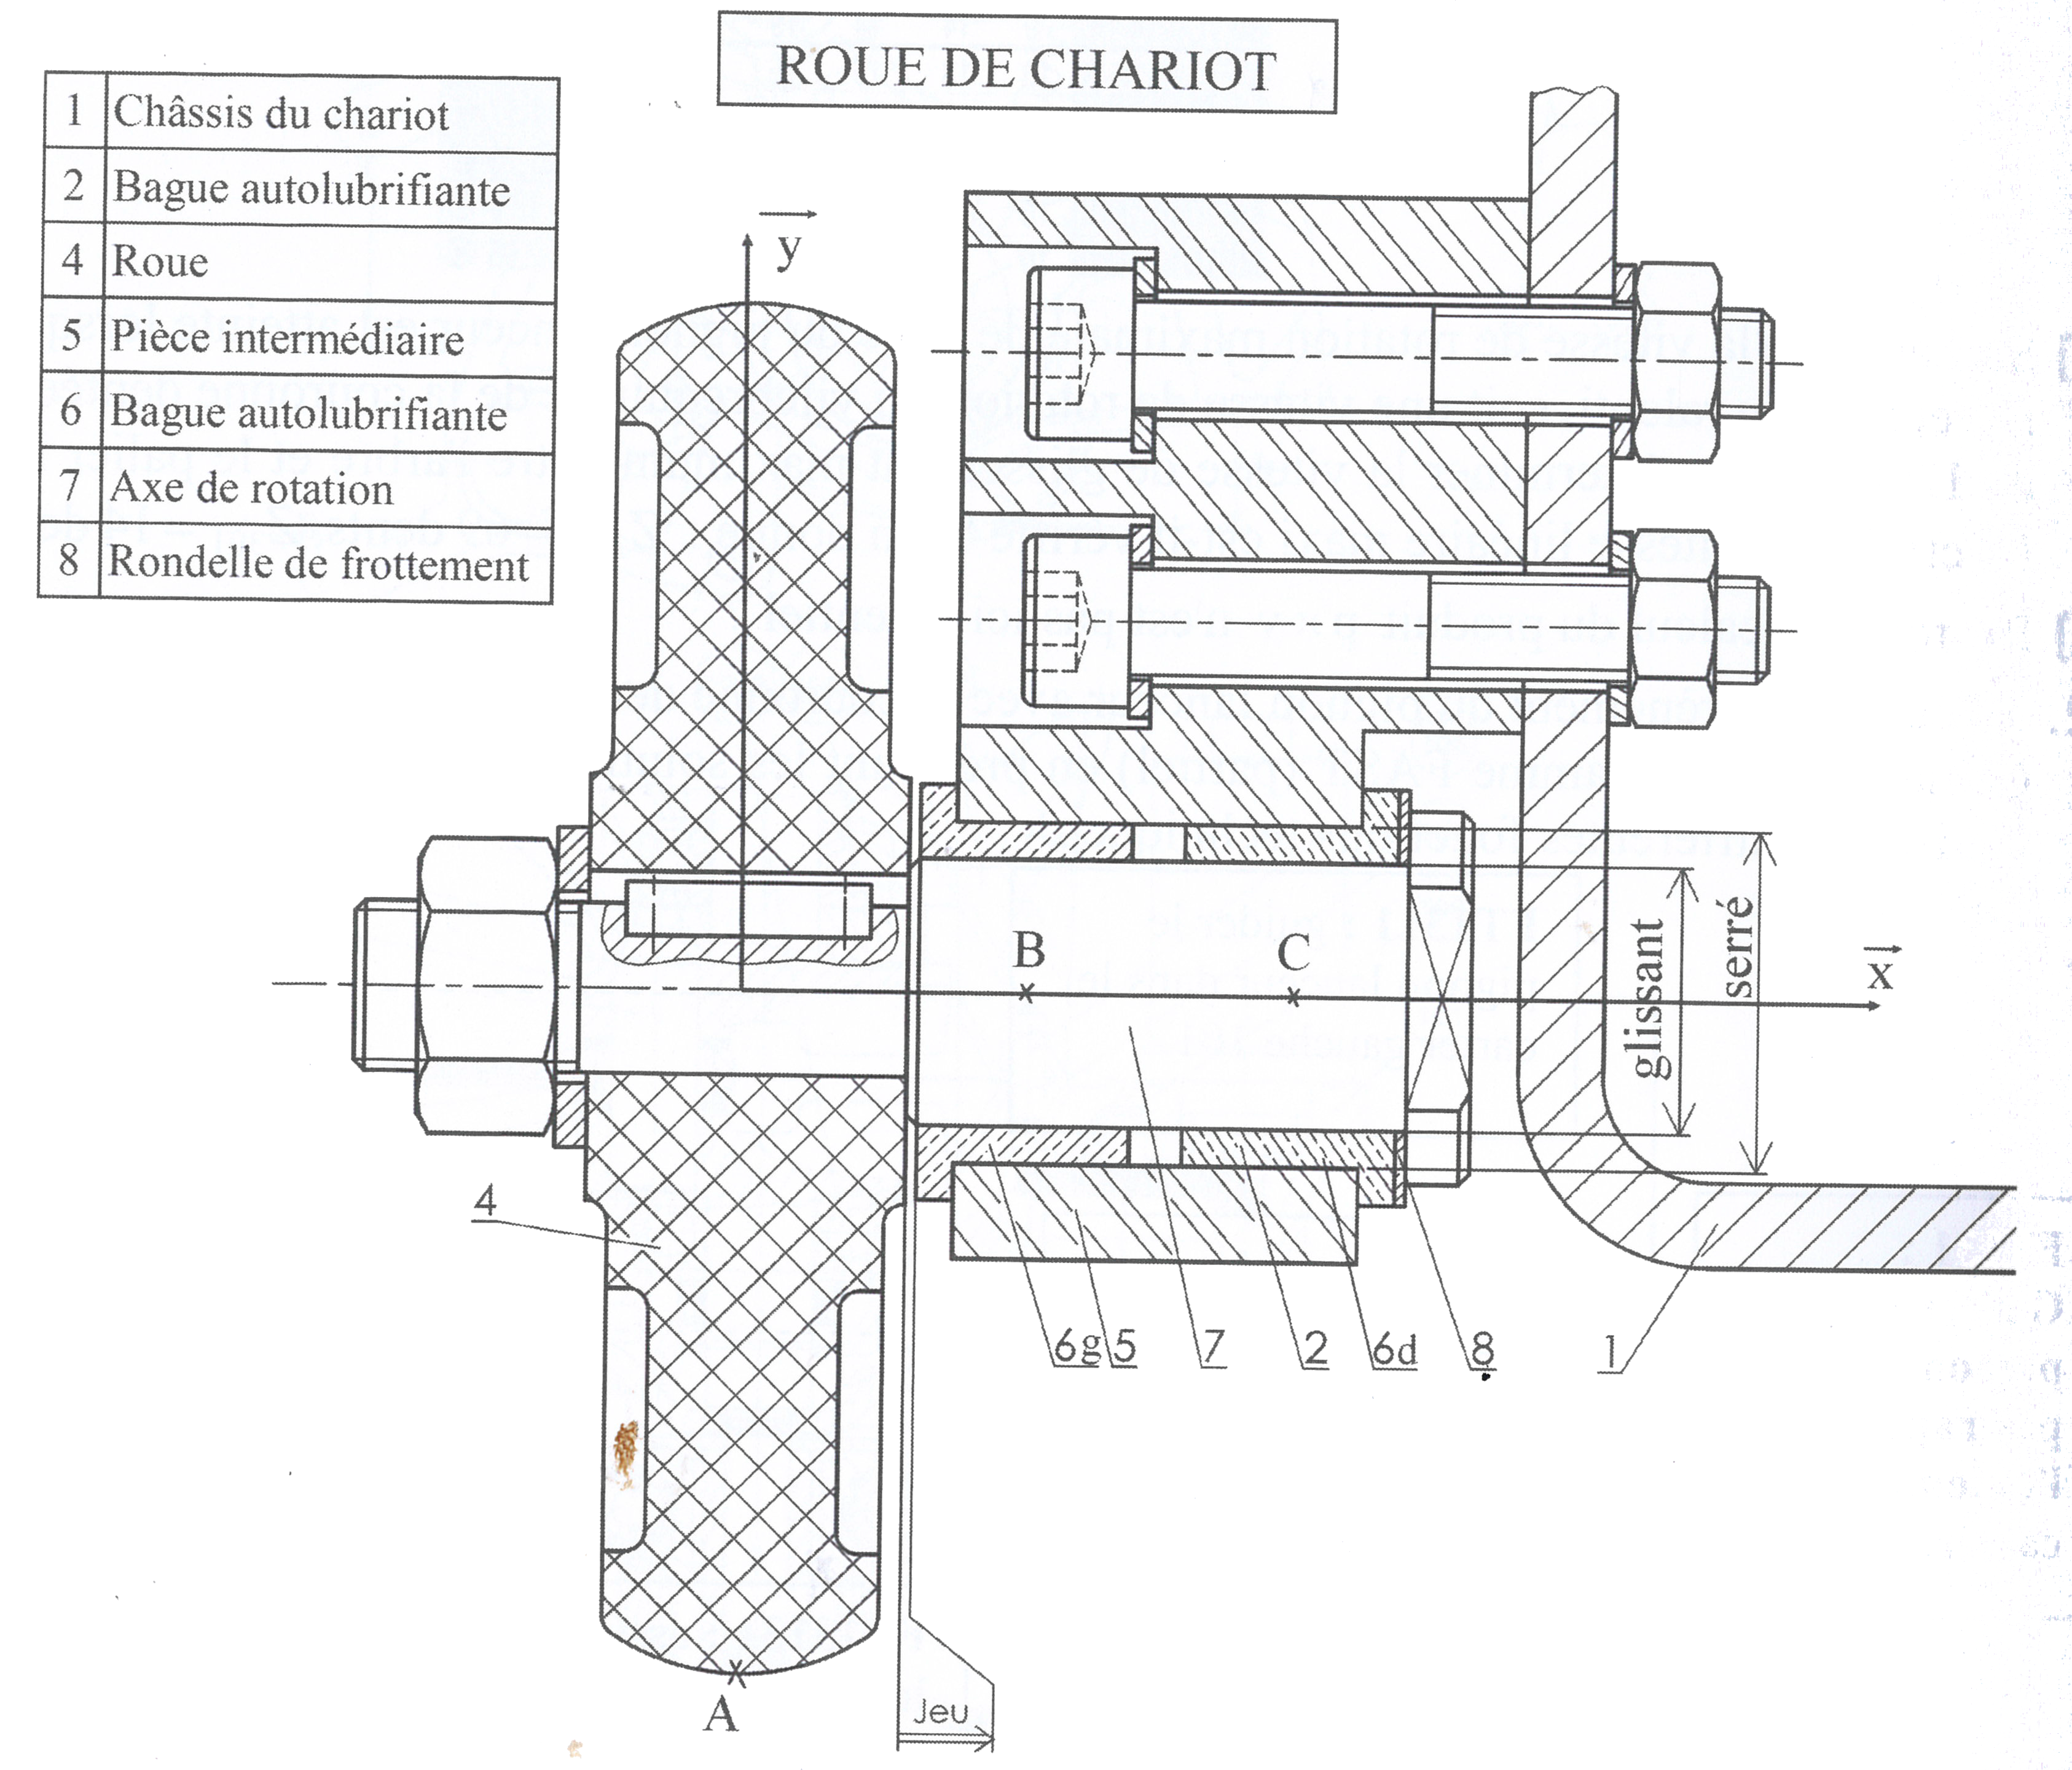
\includegraphics[width=.9\textwidth]{png/fig4}
\end{center}
\end{minipage}


\begin{center}
\includegraphics[width=.45\textwidth]{png/fig5_1}
\includegraphics[width=.45\textwidth]{png/fig5_2}
\end{center}

\section*{Nomenclature}

\begin{center}
\includegraphics[width=.9\textwidth]{png/fig6}
\end{center}


\section*{Travail demandé}

On se propose dans ce TD de réaliser la représentation 2D de différents éléments de la pince préhenseur Schrader en utilisant les projections orthogonales. On s’intéresse plus particulièrement aux éléments suivants :

\begin{center}
\includegraphics[width=.9\textwidth]{png/fig7}
\end{center}


\paragraph{}
\textit{En vous aidant des modèles numériques de chaque pièce, et des représentations en perspectives, compléter les vues extérieures incomplètes sur les dessins de définition proposés.}

\paragraph{}
\textit{Identifiez en les coloriant, chacune de ces pièces sur le dessin d’ensemble de la pince.}


\begin{center}
\includegraphics[height=\textheight]{png/fig8}
\end{center}

\begin{center}
\includegraphics[height=\textheight]{png/fig9}
\end{center}

%\begin{center}
%\includegraphics[height=\textheight]{png/fig10}
%\end{center}

\begin{center}
\includegraphics[height=\textheight]{png/fig11}
\end{center}

\begin{center}
\includegraphics[height=\textheight]{png/fig12}
\end{center}

\begin{center}
\includegraphics[height=\textheight]{png/fig13}
\end{center}

\begin{center}
\includegraphics[height=\textheight]{png/fig14}
\end{center}


\begin{center}
\includegraphics[height=\textheight]{png/plan}
\end{center}

\end{document}